\documentclass[a4paper,14pt,oneside,final]{extarticle}
\usepackage[top=2cm, bottom=2cm, left=3cm, right=1cm]{geometry}
\usepackage{scrextend}

\usepackage[T2A,T1]{fontenc}
\usepackage[ukrainian,russian,english]{babel}
\usepackage{tempora}
\usepackage{fontspec}
\setmainfont{tempora}

% Зачем: Отключает использование изменяемых межсловных пробелов.
% Почему: Так не принято делать в текстах на русском языке.
\frenchspacing

\usepackage{indentfirst}
\setlength{\parindent}{1.25cm}
\renewcommand{\baselinestretch}{1.5}

% Header
\usepackage{fancyhdr}
\pagestyle{fancy}
\fancyhead{}
\fancyfoot{}
\fancyhead[R]{\small \selectfont \thepage}
\renewcommand{\headrulewidth}{0pt}

% Captions
\usepackage{chngcntr}
\counterwithin{figure}{section}
\counterwithin{table}{section}
\usepackage[tableposition=top]{caption}
\usepackage{subcaption}
\DeclareCaptionLabelFormat{gostfigure}{Рисунок #2}
\DeclareCaptionLabelFormat{gosttable}{Таблиця #2}
\DeclareCaptionLabelSeparator{gost}{~---~}
\captionsetup{labelsep=gost}
\captionsetup[figure]{labelformat=gostfigure}
\captionsetup[table]{labelformat=gosttable}
\renewcommand{\thesubfigure}{\asbuk{subfigure}}

% Sections
\usepackage[explicit]{titlesec}
\newcommand{\sectionbreak}{\clearpage}

\titleformat{\section}
  {\centering}{\thesection \quad}{0pt}{\MakeUppercase{#1}}
\titleformat{\subsection}[block]
  {\bfseries}{\thesubsection \quad #1}{0cm}{}

\titlespacing{\section} {0cm}{0cm}{21pt}
\titlespacing{\subsection} {\parindent}{21pt}{0cm}
\titlespacing{\subsubsection} {\parindent}{0cm}{0cm}

% Lists
\usepackage{enumitem}
\renewcommand\labelitemi{--}
\setlist[itemize]{noitemsep, topsep=0pt, wide}
\setlist[enumerate]{noitemsep, topsep=0pt, wide, label=\arabic*}
\setlist[description]{labelsep=0pt, noitemsep, topsep=0pt, leftmargin=2\parindent, labelindent=\parindent, labelwidth=\parindent, font=\normalfont}

% Toc
\usepackage{tocloft}
\tocloftpagestyle{fancy}
\renewcommand{\cfttoctitlefont}{}
\setlength{\cftbeforesecskip}{0pt}
\renewcommand{\cftsecfont}{}
\renewcommand{\cftsecpagefont}{}
\renewcommand{\cftsecleader}{\cftdotfill{\cftdotsep}}

\usepackage{float}
\usepackage{pgfplots}
\usepackage{graphicx}
\usepackage{multirow}
\usepackage{amssymb,amsfonts,amsmath,amsthm}
\usepackage{csquotes}

\usepackage{listings}
\lstset{basicstyle=\footnotesize\ttfamily,breaklines=true}
\lstset{language=Matlab}

\usepackage[
	backend=biber,
	sorting=none,
	language=auto,
	autolang=other
]{biblatex}
\DeclareFieldFormat{labelnumberwidth}{#1}

% Copied from
% https://github.com/cansik/kotlin-latex-listing
% big thanks to him!
\lstdefinelanguage{Kotlin}{
  keywords={package, as, as?, typealias, this, super, val, var, fun, for, null, true, false, is, in, throw, return, break, continue, object, if, try, else, while, do, when, class, interface, enum, object, companion, override, public, private, get, set, import, abstract, vararg, expect, actual, where, suspend, data, internal, dynamic, final, by},
  keywordstyle=\color{NavyBlue}\bfseries,
  ndkeywords={@Deprecated, @JvmName, @JvmStatic, @JvmOverloads, @JvmField, @JvmSynthetic, Iterable, Int, Long, Integer, Short, Byte, Float, Double, String, Runnable, Array},
  ndkeywordstyle=\color{BurntOrange}\bfseries,
  emph={println, return@, forEach, map, mapNotNull, first, filter, firstOrNull, lazy, delegate},
  emphstyle={\color{OrangeRed}},
  identifierstyle=\color{black},
  sensitive=true,
  commentstyle=\color{gray}\ttfamily,
  comment=[l]{//},
  morecomment=[s]{/*}{*/},
  stringstyle=\color{ForestGreen}\ttfamily,
  morestring=[b]",
  morestring=[s]{"""*}{*"""},
}


\newcommand{\labnumber}{4} % fourth lab
\documentclass[a4paper,14pt,oneside,final]{extarticle}
\usepackage[top=2cm, bottom=2cm, left=3cm, right=1cm]{geometry}
\usepackage{scrextend}

\usepackage[T2A,T1]{fontenc}
\usepackage[ukrainian,russian,english]{babel}
\usepackage{tempora}
\usepackage{fontspec}
\setmainfont{tempora}

% Зачем: Отключает использование изменяемых межсловных пробелов.
% Почему: Так не принято делать в текстах на русском языке.
\frenchspacing

\usepackage{indentfirst}
\setlength{\parindent}{1.25cm}
\renewcommand{\baselinestretch}{1.5}

% Header
\usepackage{fancyhdr}
\pagestyle{fancy}
\fancyhead{}
\fancyfoot{}
\fancyhead[R]{\small \selectfont \thepage}
\renewcommand{\headrulewidth}{0pt}

% Captions
\usepackage{chngcntr}
\counterwithin{figure}{section}
\counterwithin{table}{section}
\usepackage[tableposition=top]{caption}
\usepackage{subcaption}
\DeclareCaptionLabelFormat{gostfigure}{Рисунок #2}
\DeclareCaptionLabelFormat{gosttable}{Таблиця #2}
\DeclareCaptionLabelSeparator{gost}{~---~}
\captionsetup{labelsep=gost}
\captionsetup[figure]{labelformat=gostfigure}
\captionsetup[table]{labelformat=gosttable}
\renewcommand{\thesubfigure}{\asbuk{subfigure}}

% Sections
\usepackage[explicit]{titlesec}
\newcommand{\sectionbreak}{\clearpage}

\titleformat{\section}
  {\centering}{\thesection \quad}{0pt}{\MakeUppercase{#1}}
\titleformat{\subsection}[block]
  {\bfseries}{\thesubsection \quad #1}{0cm}{}

\titlespacing{\section} {0cm}{0cm}{21pt}
\titlespacing{\subsection} {\parindent}{21pt}{0cm}
\titlespacing{\subsubsection} {\parindent}{0cm}{0cm}

% Lists
\usepackage{enumitem}
\renewcommand\labelitemi{--}
\setlist[itemize]{noitemsep, topsep=0pt, wide}
\setlist[enumerate]{noitemsep, topsep=0pt, wide, label=\arabic*}
\setlist[description]{labelsep=0pt, noitemsep, topsep=0pt, leftmargin=2\parindent, labelindent=\parindent, labelwidth=\parindent, font=\normalfont}

% Toc
\usepackage{tocloft}
\tocloftpagestyle{fancy}
\renewcommand{\cfttoctitlefont}{}
\setlength{\cftbeforesecskip}{0pt}
\renewcommand{\cftsecfont}{}
\renewcommand{\cftsecpagefont}{}
\renewcommand{\cftsecleader}{\cftdotfill{\cftdotsep}}

\newcommand{\khpistudentgroup}{КН-34г}
\newcommand{\khpistudentname}{Чепурний~А.~С.}

\newcommand{\khpidepartment}{Програмна інженерія та інформаційні технології управління}
\newcommand{\khpititlewhat}{
	Лабораторна робота №\labnumber \\
	з предмету <<Моделювання систем>>
}
\newcommand{\khpititlewho}{
	Виконав: \\
	\hspace*{\parindent} ст. групи \khpistudentgroup \\
	\hspace*{\parindent} \khpistudentname \\
	Перевірила: \\
	\hspace*{\parindent} ст. в. каф. ПІІТУ \\
	\hspace*{\parindent} Єршова~С.~І. \\
	\hspace*{\parindent} ас. каф. ПІІТУ \\
	\hspace*{\parindent} Литвинова~Ю.~С. \\
}



\lstset{language=Kotlin}
\graphicspath{{figures/}}

\begin{document}
\Ukrainian

\begin{titlepage}

\begin{center}
	МІНІСТЕРСТВО ОСВІТИ І НАУКИ УКРАЇНИ \\
	НАЦІОНАЛЬНИЙ ТЕХНІЧНИЙ УНІВЕРСИТЕТ \\
	«ХАРКІВСЬКИЙ ПОЛІТЕХНІЧНИЙ ІНСТИТУТ» \\[0.5cm]
	Кафедра <<\khpidepartment>> \\
\end{center}

\vspace{6cm}

\begin{center}
	\khpititlewhat
\end{center}

\vspace{3cm}

\begin{addmargin}[10cm]{0cm}
	\khpititlewho
\end{addmargin}

\vspace{\fill}

\begin{center}
	Харків \the\year
\end{center}

\end{titlepage}

\addtocounter{page}{1}

\section*{Розробка програмного забезпечення для моделювання неперервних детермінованих систем}
\subsubsection*{Мета роботи}
Отримати практичні навички реалізації математичних
моделей за допомогою програмного забезпечення.
\subsubsection*{Хід роботи}
\begin{enumerate}
\item Визначити засоби та технології розробки програмного коду для моделювання системи за індивідуальним завданням.
Обґрунтувати свій вибір.
\item Розробити програмний код з урахуванням вимог програмної інженерії.
\item Задокументувати результати конструювання програмного забезпечення, використовуючи візуальну нотацію Visual Paradigm for UML.
\item Оформити звіт, який повинен містити:
\begin{itemize}
\item обґрунтування вибору засобів реалізації програмного забезпечення;
\item опис обраної моделі життєвого циклу програмного забезпечення;
\item результати використання можливостей нотації Visual Paradigm for UML для документування програмного забезпечення;
\item фрагменти програмного коду, які пов'язані з реалізацією базової функціональності програмного забезпечення.
\end{itemize}
\end{enumerate}

\subsection{Вибір засобів реалізації програмного забезпечення}
Платформою для розробки застосунку було обрано ОС Android через те, що моделювання данного експерименту не потребую значної кількості ресурсів та може бути виконано на мобільному присторою.

\subsubsection{Мова програмування Kotlin}
Kotlin --- статично типізована мова програмування, що працює поверх JVM і розробляється компанією JetBrains.
Kotlin входить в список офіційно підтримуваних мов для розробки додатків для платформи Android.

\subsubsection{Середовище програмування Android Studio}
Android Studio побудоване на базі вихідного коду продукту IntelliJ IDEA Community Edition, що розвивається компанією JetBrains. 
Android Studio розвивається в рамках відкритої моделі розробки та поширюється під ліцензією Apache 2.0.
Середовище розробки адаптоване для виконання типових завдань, що вирішуються в процесі розробки застосунків для платформи Android.

Деякими з особливостей середовища є:
\begin{itemize}
\item живі макети (layout);
\item консоль розробника;
\item Android-орієнтований рефакторинг та швидкі виправлення;
\item Lint утиліти для охоплення продуктивності, юзабіліті, сумісності версій та інших проблем.
\end{itemize}

\subsubsection{База даних SQLite}
SQLite --- полегшена реляційна система керування базами даних.

Особливістю SQLite є те, що вона не використовує парадигму клієнт-сервер, тобто SQLite не є окремим процесом, з яким взаємодіє застосунок, а надає бібліотеку, з якою програма компілюється і рушій стає складовою частиною програми. 
Таким чином, як протокол обміну використовуються виклики функцій (API) бібліотеки SQLite. Такий підхід зменшує накладні витрати, час відгуку і спрощує програму. 
SQLite зберігає всю базу даних (включаючи визначення, таблиці, індекси і дані) в єдиному стандартному файлі на тому комп'ютері, на якому виконується застосунок. 
Простота реалізації досягається за рахунок того, що перед початком виконання транзакції весь файл, що зберігає базу даних, блокується; ACID-функції досягаються зокрема за рахунок створення файлу-журналу.

SQLite нативно підримується системою Android.

\subsubsection{Система керування версіями файлів Git}
Git є однією з найефективніших, надійних і високопродуктивних систем керування версіями, що надає гнучкі засоби нелінійної розробки, що базуються на відгалуженні і злитті гілок. 
Для забезпечення цілісності історії та стійкості до змін заднім числом використовуються криптографічні методи.

\subsection{Спіральна модель життєвого циклу програмного забезпечення}
Дана модель життєвого циклу допускає аналіз продукту на витку розробки, його перевірку, оцінку правильності та прийняття рішення про перехід на наступний виток або повернення на попередній виток для доопрацювання на ньому проміжного продукту~(рисунок~\ref{fig:spiral_model}).

\begin{figure}[H]
  \centering
    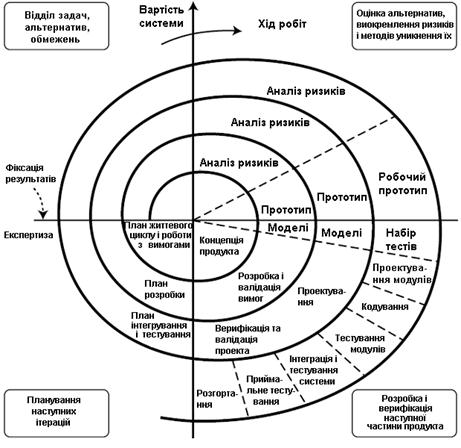
\includegraphics[width=0.7\textwidth]{spiral_model}
  \caption{Діаграма класів}
  \label{fig:spiral_model}
\end{figure}

Розробка ітераціями відображає об'єктивно існуючий спіральний цикл створення системи. 
Неповне завершення робіт на кожному етапі дозволяє переходити на наступний етап, не чекаючи повного завершення роботи на поточному. 
При ітеративному способі розробки відсутню роботу можна буде виконати на наступній ітерації. 
Головне ж завдання --- щонайшвидше показати користувачам системи та викладачу працездатний продукт, тим самим активізуючи процес уточнення і доповнення вимог.

\subsection{Фрагменти програмного коду}
Вихідний код класу \texttt{ExperimentDao}:
\lstinputlisting{code/experiment_dao.kt}

Вихідний код класу \texttt{Experiment}:
\lstinputlisting{code/experiment.kt}

Вихідний код класу \texttt{PlotView}:
\lstinputlisting{code/plot_view.kt}

\end{document}
